% !TEX root = ../../../main.tex

\toggletrue{image}
\toggletrue{imagehover}
\chapterimage{the_history_of_unicode_2x}
\chapterimagetitle{\uppercase{The History of Unicode}}
\chapterimageurl{https://xkcd.com/1953/}
\chapterimagehover{\footnotesize 2048: "Great news for Maine—we're once again an independent state!!! Thanks, @unicode, for ruling in our favor and sending troops to end New Hampshire's annexation.\protect
\includegraphics[scale=0.2]{xkcd_title_emojis}"}

\chapter{Textcodierungen}
\label{chapter-textcodierungen}

Auch Buchstaben, Satzzeichen und Emojis müssen durch Nullen und Einsen codiert werden. Nur so kann der Computer Texte, wie man Sie aus z.B. einer WhatsApp Nachricht kennt, verstehen und verschicken. Wir möchten in diesem Kapitel nun Codes anschauen, welche häufig im Zusammenhang mit Texten zum Einsatz kommen. Ziel jeder Textcodierung ist es, dass man den Text in einer Textdatei auf dem Computer abspeichern kann. Die Lernziele für dieses Kapitel lauten wie folgt:

\newcommand{\textcodierungenLernziele}{
\protect\begin{todolist}
\item Sie erklären, warum es für gewisse Codierungen einen Standard gibt.
\item Sie nennen und erklären bekannte Codes.
\item Sie codieren Text und decodieren Code-Wörter.
\end{todolist}
}

\lernziel{\autoref{chapter-textcodierungen}, \nameref{chapter-textcodierungen}}{\protect\textcodierungenLernziele}

\textcodierungenLernziele

Ein Textcode wird auch \textbf{Zeichencodierung} (eng. character encoding) genannt.

\section{Warum werden Codes standardisiert?}

Grundlegend gilt für alle Codes, dass beim Datenaustausch (siehe \autoref{figure-datenaustausch}) zwischen zwei Computern, sowohl der Sender als auch der Empfänger den gleichen Code benutzen müssen. Sonst kann der Empfänger die Daten nicht erfolgreich decodieren.

\begin{figure}[htb]
\centering
\begin{minipage}{0.15\textwidth}
\centering
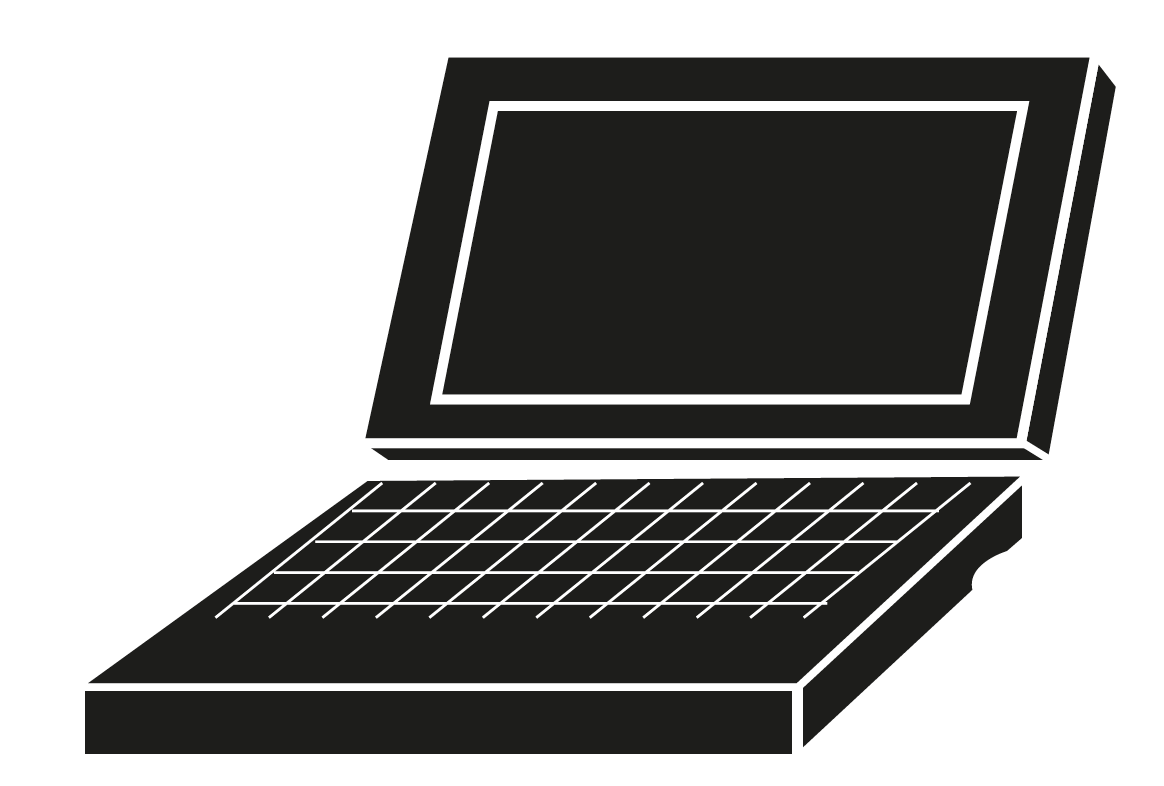
\includegraphics[scale=0.1]{notebook}
\end{minipage}
$\overbrace{\Longleftrightarrow}^{\texttt{010011010010}}$
\begin{minipage}{0.15\textwidth}
\centering
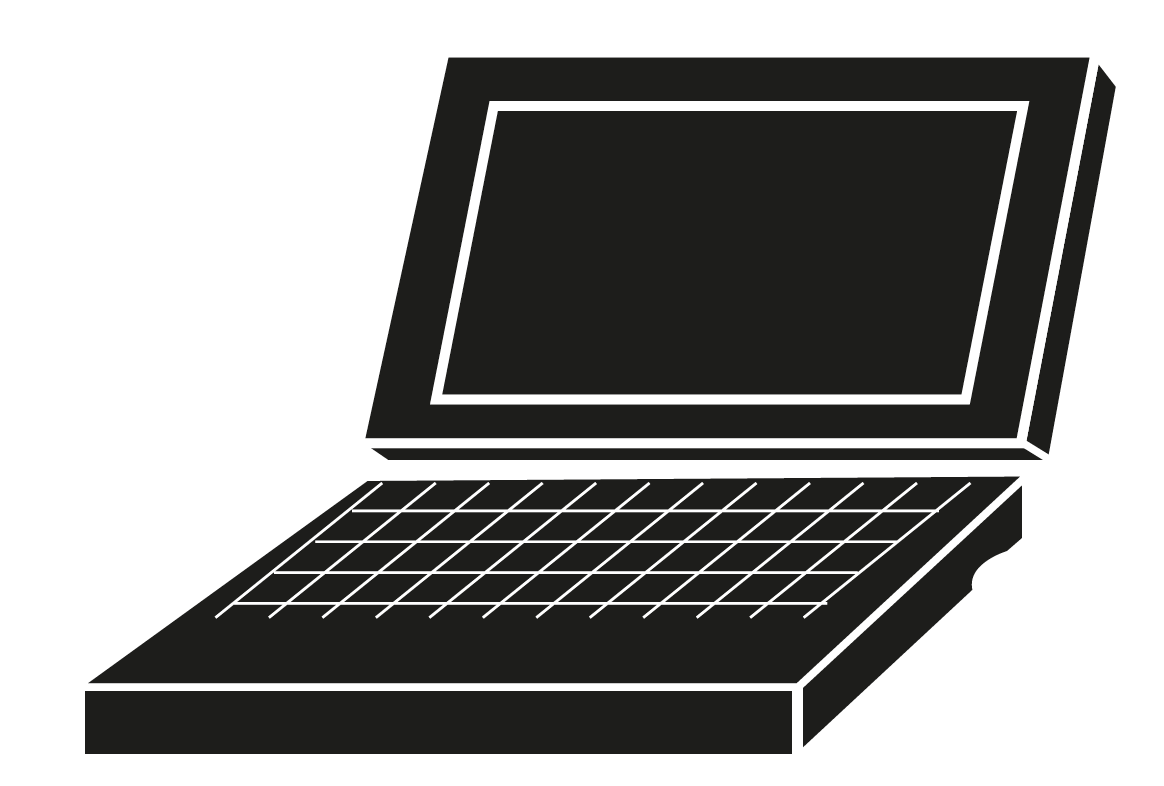
\includegraphics[scale=0.1]{notebook}
\end{minipage}
\caption{Zwei Computer tauschen Daten aus.}
\label{figure-datenaustausch}
\end{figure}

Sender und Empfänger müssen also einen Code vereinbaren. Damit nicht jeder seinen eigenen Code vereinbaren muss, gibt es verschiedene \textbf{Standards} für Codes. Die Standards für die Codierung stehen allen Programmen frei zur Verfügung und sollen die Kommunikation erleichtern. Wir schauen uns in den folgenden Abschnitten einige Standards an.

\begin{hinweis}
Ein Standard (auch Norm) genannt gibt es auch in anderen Gebieten. Es gibt zum Beispiel standardisierte Papierformate (z.B. \ac{DIN} A4) oder Buchnummern (geregelt durch die Internationale Organisation für Normung\footnote{Meist als ISO (von griechisch isos (dt. gleich)) bezeichnet.}). Standards befinden sich auch in einem Entwicklungsprozess. Ein Beispiel dafür ist die Entwicklung eines einheitlichen Ladekabels für Handys. Manchmal gibt es auch Standards die in Konkurrenz zueinander stehen (zum Beispiel \ac{HDMI} und DisplayPort zur Übertragung von Bild und Ton). \autoref{figure-xkcd-927} parodiert die Idee von Standards.
\end{hinweis}

\begin{figure}[htb]
\centering
\caption*{\uppercase{Standards} (\url{https://xkcd.com/927/})}
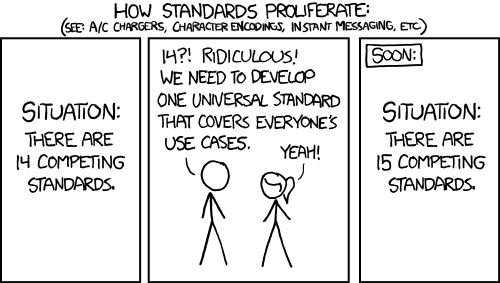
\includegraphics[scale=0.4]{standards}
\caption{Fortunately, the charging one has been solved now that we've all standardized on mini-USB. Or is it micro-USB? Shit.}
\label{figure-xkcd-927}
\end{figure}

\section{\acs{ASCII}}

Der \acl{ASCII} (\acs{ASCII}) umfasst das lateinische Alphabet (Gross- und Kleinbuchstaben), die zehn Dezimalziffern, Satzzeichen, Leerzeichen und weitere Sonderzeichen (z.B. das Dollar-Zeichen $\$$). Die Zeichen bilden im Wesentlichen die Tasten einer englischen Tastatur (US-Layout) ab. 

\subsection{Steuerzeichen}

Neben den \say{sichtbaren} Zeichen (man sagt druckbare Zeichen, da der Drucker diese auf ein Blatt Papier drucken kann\footnote{Das Leerzeichen wird auch durch den Drucker abgedeckt, in dem er für das Zeichen nichts druckt}), gibt es auch noch Steuerzeichen. Steuerzeichen sind spezielle Zeichen und können nicht dargestellt werden. Der Drucker kann Sie nicht \say{ausdrucken}. Früher wurden die Steuerzeichen zur Steuerung von Geräten (z.B. Drucker oder Fernschreiber) verwendet. Heute werden nur noch wenige Steuerzeichen verwendet. Die wichtigsten Steuerzeichen sind:

\begin{itemize}
\item ACK (Acknowledge): Empfangsbestätigung einer Nachricht.
\item BS (Backspace): Rücksetzen des Cursors.
\item HT (Horizontal Tab): \say{Tabulator-Taste}.
\item LF (Line Feed): Zeilenvorschub (Sprung in die nächste Zeile).
\item CR (Carriagee Return):  Wagenrücklauf (Sprung zum Beginn der Zeile).
\item ESC (Escape): Abbruch, Trennung, Umschaltung.
\item DEL (Delete): Löschen.
\end{itemize}

\subsection{Zeichensatz}

Bei \ac{ASCII} gibt es insgesamt $33$ Steuerzeichen und $95$ druckbare Zeichen. Der Zeichensatz von \ac{ASCII} beträgt somit 128 Zeichen.

\begin{definition}[Zeichensatz]
Der Zeichenvorrat, das heisst die Menge der möglichen Zeichen, die ein Code für die Codierung zur Verfügung stellt, bezeichnen wir als Zeichensatz.
\end{definition}

\autoref{table-ascii} zeigt alle Zeichen und die dazugehörigen Code-Wörter. \ac{ASCII} ist ein \textbf{binärer Blockcode} mit $7$ Bits. Der Code wurde in den 1960er-Jahren entwickelt und wird auch heute noch eingesetzt.

\begin{table}[!htbp]
\centering
\begin{tabular}{|c|r|r||c|r|r||r|r|r|}
\hline
Zeichen & Dez & Code-Wort & Zeichen & Dez & Code-Wort & Zeichen          & Dez & Code-Wort \\ \hline
\hline
NUL     & 0       	& 0000000     & +       & 43      		& 0101011           & V                & 86      	& 1010110           \\ \hline
SOH     & 1       & 0000001         & ,       & 44     		& 0101100          & W                & 87      	& 1010111         \\ \hline
STX     & 2       	& 0000010        & -       & 45      		& 0101101          & X                & 88      	& 1011000          \\ \hline
ETX     & 3       	& 0000011        & .       & 46      		& 0101110         & Y                & 89      	& 1011001          \\ \hline 
EOT     & 4       	& 0000100          & /       & 47   		& 0101111          & Z                & 90      	& 1011010          \\ \hline
ENQ     & 5       & 0000101          & 0       & 48   		& 0110000          & [                & 91      	& 1011011          \\ \hline
ACK     & 6       & 0000110           & 1       & 49  		& 0110001          & \textbackslash   & 92  	& 1011100          \\ \hline
BEL     & 7       	& 0000111          & 2       & 50  		& 0110010          & ]                & 93      	& 1011101          \\ \hline
BS      & 8       	& 0001000         & 3       & 51   		& 0110011          & \textasciicircum & 94   	& 1011110          \\ \hline
HT     & 9       	& 0001001          & 4       & 52  		& 0110100          & \_               & 95      	& 1011111         \\ \hline
LF      & 10      	& 0001010           & 5       & 53      	& 0110101          & `                & 96      	& 1100000          \\ \hline
VT      & 11      	& 0001011          & 6       & 54      	& 0110110          & a                & 97      	& 1100001          \\ \hline
FF      & 12      	& 0001100         & 7       & 55      	& 0110111          & b                & 98      	& 1100010         \\ \hline
CR      & 13      	& 0001101           & 8       & 56      	& 0111000          & c                & 99      	& 1100011          \\ \hline
SO      & 14      	& 0001110          & 9       & 57      	& 0111001          & d                & 100     	& 1100100          \\ \hline
SI      & 15      	& 0001111          & :       & 58      	& 0111010          & e                & 101     	& 1100101          \\ \hline
DLE     & 16      & 0010000         & ;       & 59      	& 0111011          & f                & 102     	& 1100110          \\ \hline
DC1     & 17      & 0010001          & <       & 60      	& 0111100          & g                & 103     	& 1100111          \\ \hline
DC2     & 18      & 0010010          & =       & 61      	& 0111101          & h                & 104     	& 1101000         \\ \hline
DC3     & 19      & 0010011          & >       & 62      	& 0111110          & i                & 105     	& 1101001          \\ \hline
DC4     & 20      & 0010100         & ?       & 63      	& 0111111          & j                & 106     	& 1101010          \\ \hline
NAK     & 21     	& 0010101          & @       & 64      	& 1000000          & k                & 107     	& 1101011         \\ \hline
SYN     & 22     	& 0010110         & A       & 65      	& 1000001          & l                & 108     	& 1101100         \\ \hline
ETB     & 23      & 0010111          & B       & 66      	& 1000010          & m                & 109    	& 1101101         \\ \hline
CAN     & 24     & 0011000         & C       & 67      	& 1000011          & n                & 110     	& 1101110          \\ \hline
EM      & 25      	& 0011001         & D       & 68      	& 1000100          & o                & 111     	& 1101111          \\ \hline
SUB     & 26     	& 0011010         & E       & 69      	& 1000101          & p                & 112     	& 1110000          \\ \hline
ESC     & 27    	& 0011011         & F       & 70      	& 1000110          & q                & 113     	& 1110001          \\ \hline
FS      & 28      	& 0011100          & G       & 71      	& 1000111          & r                & 114     	& 1110010          \\ \hline
GS      & 29      	& 0011101          & H       & 72      	& 1001000          & s                & 115     	& 1110011         \\ \hline
RS      & 30     	& 0011110          & I       & 73      	& 1001001          & t                & 116     	& 1110100          \\ \hline
US      & 31      	& 0011111          & J       & 74      	& 1001010          & u                & 117     	& 1110101          \\ \hline
$\sqcup$ & 32 	& 0100000          & K       & 75      	& 1001011          & v                & 118     	& 1110110          \\ \hline
!       & 33      	& 0100001         & L       & 76      	& 1001100          & w                & 119     	& 1110111          \\ \hline
"       & 34      	& 0100010          & M       & 77      	& 1001101          & x                & 120     	& 1111000         \\ \hline
\#      & 35      	& 0100011          & N       & 78      	& 1001110          & y                & 121     	& 1111001          \\ \hline
\$      & 36      	& 0100100          & O       & 79      	& 1001111          & z                & 122     	& 1111010         \\ \hline
\%      & 37      	& 0100101          & P       & 80      	& 1010000          & \{               & 123     	& 1111011          \\ \hline
\&      & 38      	& 0100110          & Q       & 81      	& 1010001          & |                & 124     	& 1111100          \\ \hline
‘     & 39      	& 0100111          & R       & 82      	& 1010010          & \}               & 125     	& 1111101          \\ \hline
(       & 40      	& 0101000          & S       & 83      	& 1010011         & \textasciitilde  & 126  	& 1111110          \\ \hline
)       & 41      	& 0101001          & T       & 84      	& 1010100          & DEL                & 127     	& 1111111          \\ \hline
*       & 42      	& 0101010          & U       & 85      	& 1010101          &                  &         	&           \\ \hline
\end{tabular}
\caption{Das Zeichen $\sqcup$ soll das Leerzeichen darstellen. Die \protect\say{Dez}-Spalte (Dezimalzahl) dient zur einfacheren Kommunikation zwischen zwei Personen. Es entspricht gerade der Dezimalzahl, wenn wir die Bits als Dualzahl decodieren.}
\label{table-ascii}
\end{table}

\clearpage

\subsection{Aufgaben}
\label{subsection-ascii-aufgaben}

\begin{enumerate}
\item Codieren Sie Ihren Vornamen mit \ac{ASCII} (mindestens die ersten drei Zeichen).

\fillwithgrid{0.75in}

\item Decodieren Sie 0110010011000001100000110001011101001000001000001010000010100\\11111000011000011100011110010101000001001111110010011110011110011111001111\\001011111001 mit \ac{ASCII}.

\fillwithgrid{0.25in}

\item Warum ist bei \ac{ASCII} für jedes Code-Wort die gleiche Anzahl an Stellen vorhanden?

\fillwithgrid{0.75in}

\item Welche Zeichen sind bei \ac{ASCII} nicht vorhanden? Warum?

\fillwithgrid{0.75in}

\item Wie funktioniert die Darstellung aus \autoref{table-ascii-compact} von \ac{ASCII}? Erklären Sie mit einem Beispiel.

\fillwithgrid{0.75in}

\end{enumerate}

\begin{table}[htb]
\centering
\begin{tabular}{|c|c|c|c|c|c|c|c||c|}
\hline
\multicolumn{9}{|c|}{Bitpositionen} \\ \hline
\multicolumn{8}{|c||}{7, 6, 5} & 4, 3, 2, 1 \\ \hline \hline
000 & 001 & 010 & 011 & 100 & 101 & 110 & 111 & \\\hline 
NUL & DLE & $\sqcup$  & 0   & @   & P   &  `   &  p & 0000    \\ \hline 
SOH  & DC1   &  !   &  1   &  A   &  Q   &  a   &  q & 0001     \\ \hline 
STX   &  DC2    &   "   &   2  &  B   &  R   &  b   &  r & 0010     \\ \hline 
ETX   &  DC3    &  \#   &  3   &  C   &  S   &  c   &  s & 0011     \\ \hline 
EOT   & DC4    &  \$   &  4   &  D   &  T   &  d   &  t & 0100     \\ \hline 
ENQ  & NAK    &  \%   &  5   &  E   &  U   & e    & u & 0101      \\ \hline 
ACK  & SYN    & \&    &  6   &  F   &  V   &  f   &  v & 0110    \\ \hline 
BEL   & ETB   & ‘     &   7 &  G   &  W   &  g   &  w & 0111    \\ \hline 
BS   &  CAN   &  (    &  8   & H    & X    &  h   &  x & 1000    \\ \hline 
HT   &  EM   &  )   &  9   &  I   &  Y   &  i   &  y & 1001     \\ \hline 
LF   &  SUB   &  *   & :    &  J   &  Z   & j    & z & 1010     \\ \hline 
VT   &   ESC  &  +   & ;    &  K   &  [   & k    & \{ & 1011      \\ \hline 
FF   & FS    &  ,   & <    &  L   &  \textbackslash   &  l   &  | & 1100    \\ \hline 
CR   &  GS   &  -   & =    & M    &  ]   & m    &  \}  & 1101   \\ \hline 
SO   &  RS   &  .   &  >   &  N   &  \textasciicircum   &  n   &  \textasciitilde  & 1110   \\ \hline 
SI  &  US   &   /  &  ?   &  O   &  \_   & o    & DEL & 1111    \\ \hline
\end{tabular}
\caption{Kompakte Notation von \ac{ASCII}.}
\label{table-ascii-compact}
\end{table}

\section{Latin-1}

Da mit \ac{ASCII} nicht alle Schriftzeichen der Menschen dargestellt werden können, gibt es noch weitere Codes. Bereits für die deutsche Sprache fehlen bei \ac{ASCII} die Code-Wörter für die Umlaute (ä, ö und ü). Deshalb wurde ISO 8859 erstellt. Dies ist eine Sammlung (man sagt auch Familie) von $8$-Bit-Codes. Der Standard ISO 8859-1 Code ist besser bekannt als \textbf{Latin-1} und stellt eine Erweiterung von \ac{ASCII} dar. Der Code wird hinsichtlich einiger westeuropäischer Zeichen erweitert (z.B. à, å oder ü). 

\subsection{Zeichensatz}

Bei Latin-1 gibt es insgesamt \num{191} Zeichen. Im Vergleich zu \ac{ASCII} sind somit \num{96} Zeichen hinzugekommen. Insgesamt können \num{255} Zeichen codiert werden. Einige Code-Wörter sind freigelassen für Steuerzeichen. Pro Code-Wort werden somit \qty{8}{\bit} benutzt. Die \ac{ASCII} Code-Wörter von $0100000$ ($\sqcup$) bis $1111110$ (\textasciitilde) wurden übernommen und mit einer führenden Null ergänzt. Aus $1111110$ wird somit $01111110$. Ab $10100000$ (\ac{NBSP}) folgen dann bis $11111111$ (ÿ) die neuen Zeichen von Latin-1 (siehe \autoref{table-latin-1-compact}).

\begin{table}[htb]
\centering
\begin{tabular}{|c|c|c|c|c|c||c|}
\hline
\multicolumn{7}{|c|}{Bitpositionen} \\ \hline
\multicolumn{6}{|c||}{8, 7, 6, 5} & 4, 3, 2, 1 \\ \hline \hline
1010 & 1011 & 1100 & 1101 & 1110 & 1111 & \\\hline
NBSP & ° & À & Ð & à & ð & 0000 \\ \hline 
¡   &  ±  &  Á   &  Ñ   &  á   &   ñ & 0001  \\ \hline 
¢   &  ²   &  Â   &   Ò  &   â  &   ò   & 0010   \\ \hline 
£   &  ³   &  Ã   &   Ó  &  ã   &    ó   & 0011    \\ \hline 
¤   &  ´   &  Ä   &   Ô  &  ä  &    ô  & 0100     \\ \hline 
¥   & µ    &  Å   &  Õ  &  å   &   õ    & 0101    \\ \hline 
¦   &   ¶  &  Æ   &  Ö  &  æ  &    ö   & 0110     \\ \hline 
§   &  ·   &  Ç   &  ×   &   ç  &   ÷   & 0111     \\ \hline 
¨   &  ¸   &   È  &   Ø  & è    &   ø    & 1000    \\ \hline 
©   &  ¹   &  É   &  Ù  &  é  &  ù   & 1001   \\ \hline 
ª   & º   & Ê   &  Ú  & ê   &  ú   & 1010       \\ \hline 
«   &  »   & Ë    &  Û   &  ë   &  û   & 1011      \\ \hline 
¬   &  ¼   & Ì    & Ü   & ì    &   ü   & 1100     \\ \hline 
SHY &  ½   &  Í   &  Ý   &  í   & ý   & 1101   \\ \hline 
®   &   ¾  &  Î   & Þ    &   î  &    þ   & 1110    \\ \hline 
¯   &  ¿   &  Ï   &  ß  &  ï   &   ÿ   & 1111     \\ \hline
\end{tabular}
\caption{Kompakte Notation von Latin-1.}
\label{table-latin-1-compact}
\end{table}

Latin-1 wird im \ac{WWW} und bei Textdokumenten immer seltener benutzt. \autoref{table-latin-1-usage} zeigt den Anteil der Websites die Latin-1 zur Codierung benutzen.

\begin{table}[htb]
\centering
\small
\begin{tabular}{|c|c|c|c|c|c|c|c|c|c|c|c|}
\hline
2010   & 2011   & 2012   & 2013   & 2014   & 2015  & 2016  & 2017  & 2018  & 2019  & 2020  & 2021 \\ \hline
28.6\% & 22.0\% & 17.2\% & 13.5\% & 10.8\% & 9.3\% & 6.9\% & 5.5\% & 4.3\% & 3.6\% & 1.6\% & 1.4\%       \\ \hline
\end{tabular}
\normalsize
%https://w3techs.com/technologies/history_overview/character_encoding/ms/y
\caption{Anteil der Websites, die ISO-8859-1 (Latin-1) als Codierung verwenden.}
\label{table-latin-1-usage}
\end{table}

Als De-Facto-Standard für Websites hat sich der Code aus dem nächsten Abschnitt durchgesetzt. Trotzdem hat Latin-1 seine Berechtigung. Datenbanken verwenden gerne diesen Code, da man Text kompakt speichern kann. Es braucht \say{nur} \qty{1}{\byte} pro Zeichen.

\section{Unicode}

Dieser Codierungsstandard hat das Ziel die Schriftzeichen aller Kulturen zu berücksichtigen und unter einem Dach zu vereinen. Der Code wird kontinuierlich erweitert.

\subsection{Zeichensatz}

Im September 2022 ist die Version 15.0 von Unicode erschienen. Es kamen \num{4489} neue Zeichen hinzu (darunter sind \num{20} neue Emojis) und der Code umfasst nun \num{149186} Zeichen. Unicode ist so konzipiert, dass auch in der Zukunft noch mehr Zeichen aufgenommen werden können. Der Code hat \say{Platz} für insgesamt \num{1114112} Code-Wörter. Somit sind zurzeit gut \qty{13}{\percent} benutzt.

\subsection{Code-Points}

Der Standard bezeichnet Code-Wörter als Code Points (dt. Codepunkte). Jedes Zeichen im Unicode hat einen eindeutigen Code Point. \autoref{table-unicode} zeigt fünf Zeichen aus dem Unicode und die dazugehörigen Code Points (Code-Wörter). Code Points beginnen mit den Zeichen \textbf{U+} gefolgt von der eindeutigen Nummer. Die \textbf{eindeutige Nummer} wird als \textbf{Hexadezimalcode} (siehe \autoref{chapter-hexadezimalcode}) angegeben. Der Hexadezimalcode wird gerne deshalb eingesetzt, da sich Binärzahlen so kompakt darstellen lassen und der Umgang damit für den Menschen angenehmer ist.

\begin{table}[htb]
\centering
\begin{tabular}{|c|c|c|}
\hline
Zeichen & Code Point                & Beschreibung               \\ \hline
ß       & U+00DF     & LATIN SMALL LETTER SHARP S \\ \hline
€       & U+20AC     &  EURO SIGN                  \\ \hline
©       & U+00A9     &  COPYRIGHT SIGN             \\ \hline
\rule{0pt}{15pt} 
\includegraphics[scale=0.1]{emoji_grinning_face} & U+1F600    &   GRINNING FACE       \\ \hline
A & U+0041    & LATIN CAPITAL LETTER A             \\ \hline
\end{tabular}
\caption{Code Points besitzen mindestens \num{4} Zeichen (ggf. auffüllen mit führenden Nullen).}
\label{table-unicode}
\end{table}

Unicode ist der De-Facto-Standard für Textcodierungen. Microsoft Word Dokumente, WhatsApp-Nachrichten und fast alle Websites (um nur einige Beispiele zu nennen) verwenden Unicode.

\subsection{\acs{UTF}}

Unicode definiert für jedes Zeichen einen Code Point. Dieser Code Point wird jedoch nicht direkt in Bits übersetzt. Es erfolgt eine weitere Codierung. \ac{UTF} beschreibt, wie wir einen Code Point in eine Folge von Bits übersetzen. Dabei gibt es mehrere Varianten: UTF-32, UTF-16 und UTF-8.

\subsubsection{UTF-32}

Bei UTF-32 wird jeder Code Point mit \qty{32}{\bit} $=$ \qty{4}{\byte} codiert. Wir können den Code Point für ein Zeichen somit direkt in eine Folge von Bits übersetzen. \autoref{table-utf-32} zeigt erneut die Beispiele.

\begin{table}[htb]
\centering
\begin{tabular}{|c|c|c|}
\hline
Zeichen & Code Point & UTF-32 \\ \hline
ß     	& U+00DF	& 00000000 00000000 00000000 11011111\\ \hline
€     	& U+20AC     	& 00000000 00000000 00100000 10101100\\ \hline
©     	& U+00A9     	& 00000000 00000000 00000000 10101001\\ \hline
\rule{0pt}{15pt} 
\includegraphics[scale=0.1]{emoji_grinning_face} & U+1F600	& 00000000 00000001 11110110 00000000\\ \hline
A & U+0041		& 00000000 00000000 00000000 01000001\\ \hline
\end{tabular}
\caption{Für jede Hexziffern werden \num{4} Bits benötigt. Besitzt ein Code Point weniger als \num{8} Hexziffern, dann füllen wir einfach mit Nullen auf. UTF-32 ist ein \textbf{Blockcode}.}
\label{table-utf-32}
\end{table}

\subsubsection{UTF-16}

Bei UTF-16 kommt es auf den Code Point an, wie die Codierung erfolgt. Die Code Points aus dem Bereich U+0000 bis U+D7FF und U+E000 bis U+FFFF werden direkt mit \qty{16}{\bit} codiert. Alle anderen Code Points werden durch zwei \qty{16}{\bit} Code-Wörter codiert. Somit erhält ein Code Point entweder \qty{16}{\bit} oder \qty{32}{\bit}. \autoref{table-utf-16} zeigt erneut die Beispiele.

\begin{table}[htb]
\centering
\begin{tabular}{|c|c|r|}
\hline
Zeichen & Code Point & UTF-16 \\ \hline
ß     	& U+00DF	& 00000000 11011111\\ \hline
€     	& U+20AC     	& 00100000 10101100\\ \hline
©     	& U+00A9     	& 00000000 10101001\\ \hline
\rule{0pt}{15pt} 
\includegraphics[scale=0.1]{emoji_grinning_face} & U+1F600	& 11011000 00111101 11011110 00000000\\ \hline
A & U+0041		& 00000000 01000001\\ \hline
\end{tabular}
\caption{Das Emoji wird mit \qty{32}{\bit} codiert. Die Umwandlung erfolgt mit einer mathematischen Berechnung. Für alle Code-Wörter ist eine eindeutige Decodierung garantiert.}
\label{table-utf-16}
\end{table}

UTF-16 ist gerade so konstruiert, dass die meisten Zeichen des Unicodes \say{nur} \qty{2}{\byte} benötigen. Im Vergleich zu UTF-8 (siehe nächster Abschnitt) ist dies für Zeichen aus dem asiatischen Raum von Vorteil. Für diese Zeichen reduziert sich der Speicherbedarf im Vergleich zu UTF-8. Englische Texte benötigen in der Regel mit UTF-16 einen erhöhten Speicherbedarf.

\subsubsection{UTF-8}

Die am häufigsten eingesetzte Codierung für Code Points ist UTF-8. Die Code Points werde mit \qty{1}{\byte} bis \qty{4}{\byte} codiert. Je nach Code Point werden die Code-Wörter also unterschiedlich lang. UTF-8 ist somit \textbf{kein} Blockcode. Trotzdem ist die eindeutige Decodierung garantiert. Die Codierung erfolgt nach vier Regeln (siehe \autoref{table-utf-8}), je nach dem in welchem Bereich der Code Point liegt.

\begin{table}[htb]
\centering
\begin{tabular}{|c|c|l|}
\hline
Code Point 					& Speicherbedarf	& Muster 		\\ \hline
U+0000 0000 bis U+0000 007F		& \qty{1}{\byte}      	& 0xxxxxxx      \\ \hline
U+0000 0080 bis U+0000 07FF		& \qty{2}{\byte}      	& 110xxxxx 10xxxxxx       \\ \hline
U+0000 0800 bis U+0000 FFFF	& \qty{3}{\byte}      	& 1110xxxx 10xxxxxx 10xxxxxx       \\ \hline
U+0001 0000 bis U+0010 FFFF	& \qty{4}{\byte}      	& 11110xxx 10xxxxxx 10xxxxxx 10xxxxxx       \\ \hline
\end{tabular}
\caption{Die \protect\say{x} sind Platzhalter und müssen durch die tatsächlichen Bits des Code Points von rechts nach links ersetzt werden.}
\label{table-utf-8}
\end{table}

\begin{example}
Wir codieren zwei Beispiele mit UTF-8:

\begin{itemize}
\item Der Code Point U+0041, das Zeichen A, liegt im ersten Bereich (0xxxxxxxx). Wir codieren $41_{16}$ zu $01000001_2$ und erhalten somit direkt das UTF-8 Code-Wort.
\item Der Code Point U+00DF, das Zeichen ß, liegt im zweiten Bereich. Wir codieren $DF_{16}$ zu $11011111_2$. Wir ersetzen die Platzhalter (\say{x}) von \textbf{rechts} nach \textbf{links} durch die Bits. Alle übrig gebliebenen Platzhalter werden durch eine \num{0} ersetzt.

\begin{center}
\texttt{110x xxxx 10xx xxxx} \\
\texttt{~~~~~~~11~~~01~1111} \\
\texttt{110x xx11 1001 1111} \\
\texttt{1100 0011 1001 1111} \\
\end{center}

Wir erhalten das UTF-8 Code-Wort 1100001110011111. Es besteht aus \qty{2}{\byte}.
\end{itemize}
\end{example}

\subsection{Aufgaben}
\label{subsection-unicode-aufgaben}

\begin{enumerate}
\item Codieren Sie den ersten Buchstaben (Grossbuchstabe) Ihres Vornamens mit Unicode.
\begin{enumerate}
\item Notieren Sie den Code Point (\url{unicode-table.com})
\fillwithgrid{0.25in}
\item Codieren Sie den Code Point mit UTF-32.
\fillwithgrid{0.25in}
\item Codieren Sie den Code Point mit UTF-8.
\fillwithgrid{0.25in}
\end{enumerate}
\item Codieren Sie © mit Unicode und UTF-8.
\fillwithgrid{1.5in}
\item Codieren Sie € mit Unicode und UTF-8.
\fillwithgrid{1.5in}
\item Codieren Sie \rule{0pt}{15pt} 
\includegraphics[scale=0.1]{emoji_grinning_face} mit Unicode und UTF-8.
\fillwithgrid{1.5in}
\item Folgendes UTF-32 Code-Wort ist gegeben: $00000000000000000000000001010111_{2}$. Welcher Code Point wurde hier codiert? Der Code Point codiert ein ASCII-Zeichen. Welches?
\fillwithgrid{1.5in}

\newpage

\item Folgendes UTF-8 Code-Wort ist als Hexadezimalzahl gegeben: $C384_{16}$. Welcher Code Point wurde hier codiert? Suchen Sie im Internet nach dem Zeichen für das Code-Wort.
\fillwithgrid{1.75in}
\item Folgendes UTF-8 Code-Wort ist als Hexadezimalzahl gegeben: $F09FAB95_{16}$. Welcher Code Point wurde hier codiert? Suchen Sie im Internet nach dem Zeichen für den Code Point.
\fillwithgrid{1.75in}
\item Folgendes UTF-8 Code-Wort ist als Hexadezimalzahl gegeben: $F09F8E84_{16}$. Welcher Code Point wurde hier codiert? Suchen Sie im Internet nach dem Zeichen für den Code Point.
\fillwithgrid{1.75in}
\item Vergleichen Sie die druckbaren \ac{ASCII}-Zeichen mit UTF-8. Was stellen Sie fest?
\fillwithgrid{1in}
\item Erkunden Sie sich im \ac{WWW} für welche Emoji-Kategorie keine neuen Vorschläge mehr angenommen werden. Warum?
\fillwithgrid{\stretch{1}}
\end{enumerate}